\section{A little history}

\begin{frame}{Constraints Problems}
    \begin{figure}
    \begin{centering}
    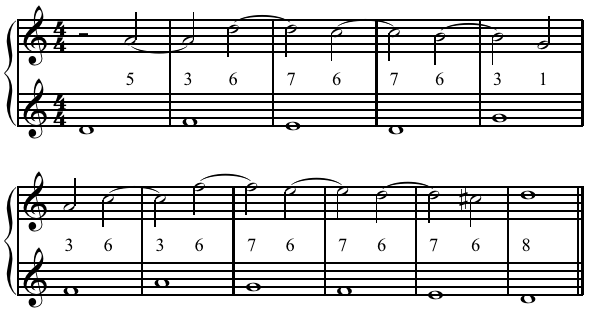
\includegraphics[height=2.25in]{assets/include-species-counterpoint.png}
    \caption{\emph{Species counterpoint}: a constraint-satisfaction-problem dream}
    \end{centering}
    \end{figure}
\end{frame}

\begin{frame}{Random Numbers}
    \begin{figure}
    \begin{centering}
    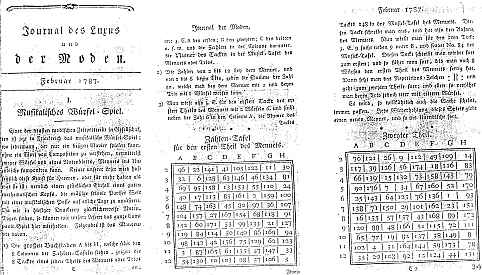
\includegraphics[height=2.25in]{assets/include-dice-game.jpg}
    \caption{Random minuets via Mozart's Dice Game}
    \end{centering}
    \end{figure}
\end{frame}

\begin{frame}{Xenakis}
    \begin{figure}
    \begin{centering}
    \begin{tabular}{cc}
    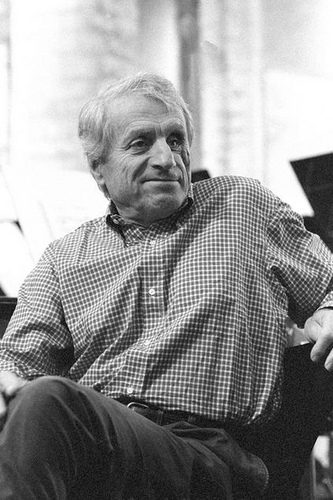
\includegraphics[height=2.25in]{assets/include-xenakis-portrait.jpg}
    &
    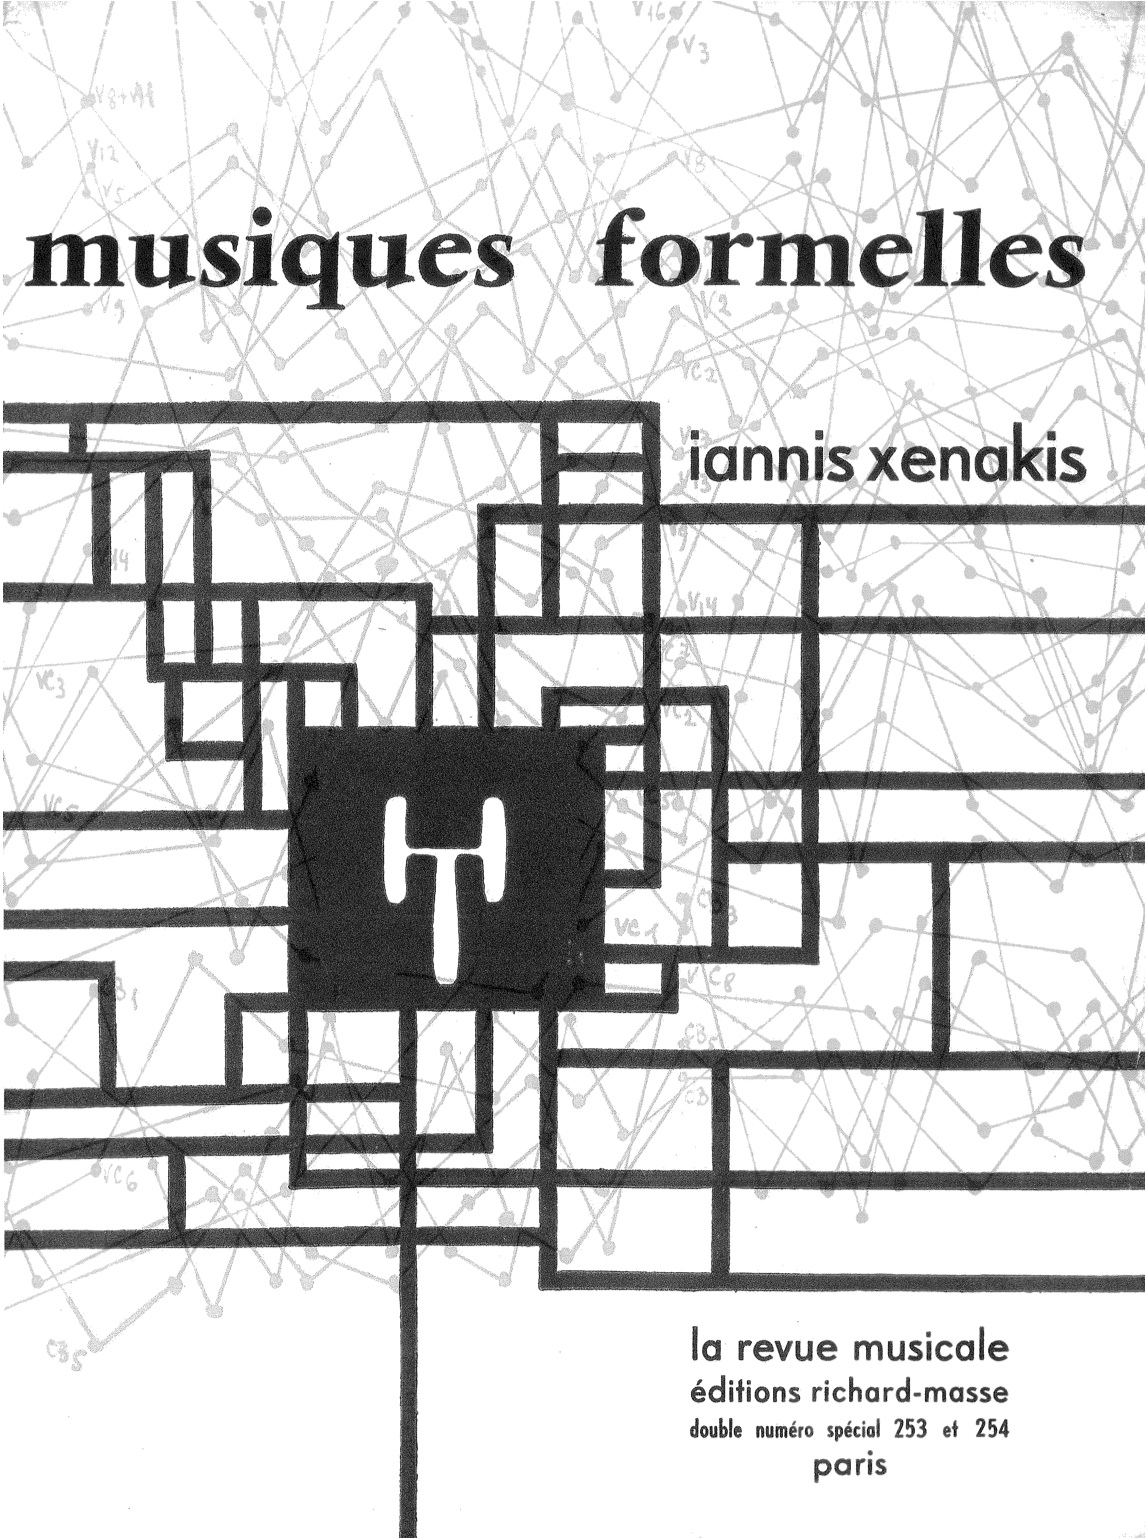
\includegraphics[height=2.25in]{assets/include-xenakis-formalized-music.jpg}
    \end{tabular}
    \caption{Iannis Xenakis (1922-2001)}
    \end{centering}
    \end{figure}
\end{frame}

\begin{frame}{Random Distributions}
    \begin{figure}
    \begin{centering}
    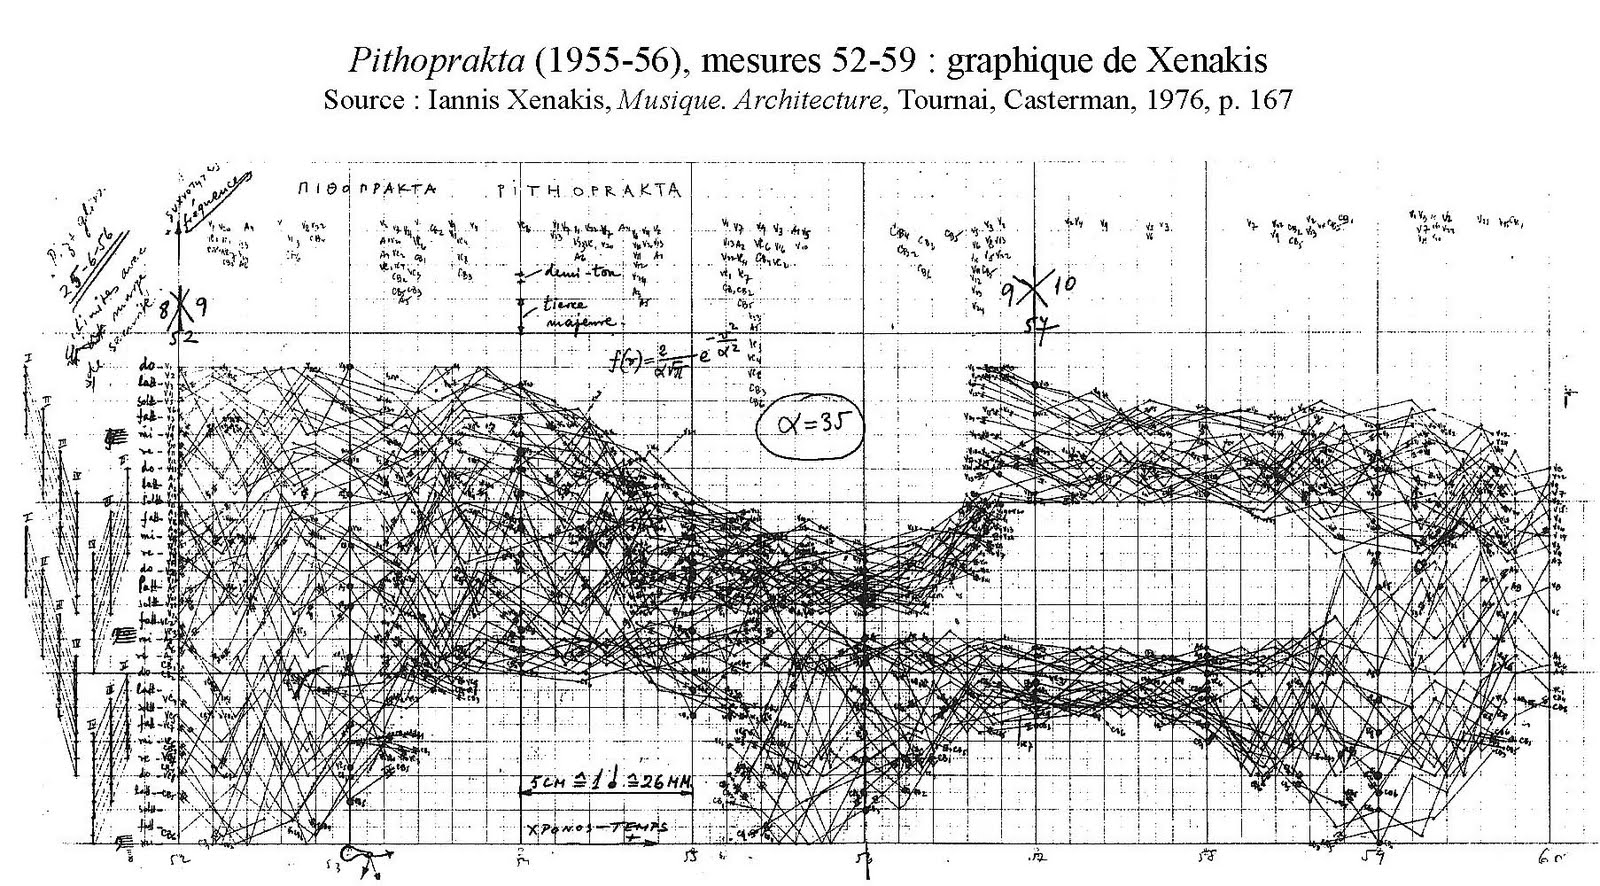
\includegraphics[max width=\linewidth]{assets/include-xenakis-pithoprakta.jpg}
    \caption{Stochastic string orchestra trajectories}
    \end{centering}
    \end{figure}
\end{frame}

\begin{frame}{Lisp, lots of Lisp, fields of Lisp, a tremendous amount of Lisp}
    \begin{figure}
    \begin{centering}
    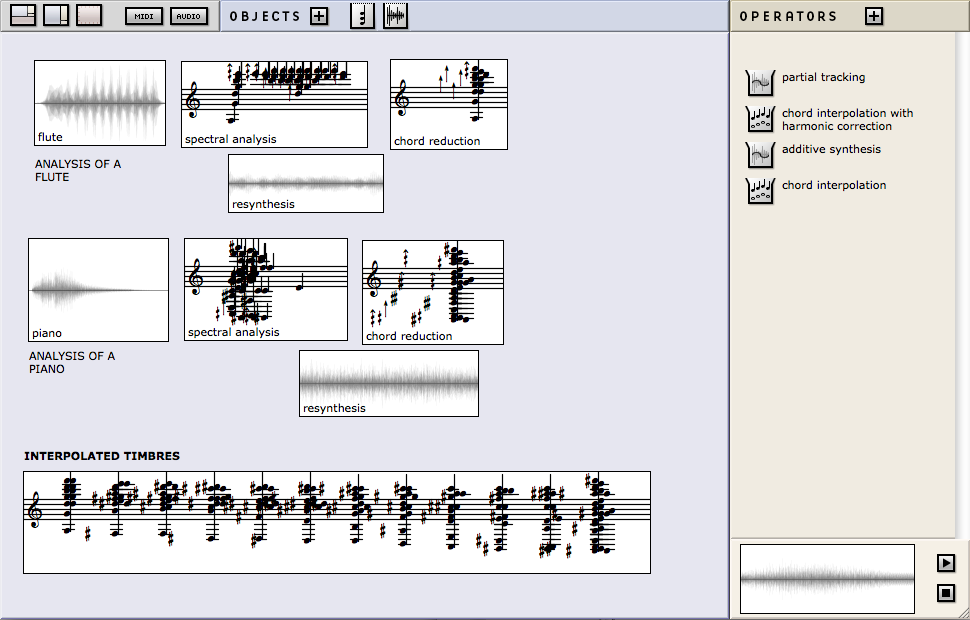
\includegraphics[height=2in]{assets/include-open-music.png}
    \caption{OpenMusic: Lisp hidden behind boxes}
    \end{centering}
    \end{figure}
\end{frame}

\begin{frame}{Yellow Lisp, red Lisp, Lisp with feathers, cream of Lisp}
    \begin{figure}
    \begin{centering}
    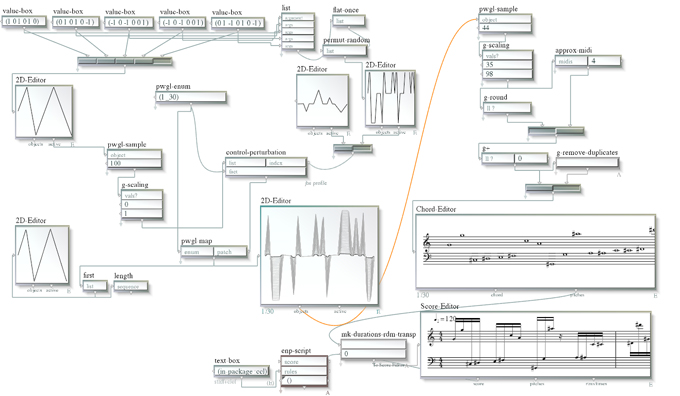
\includegraphics[height=2in]{assets/include-pwgl.jpg}
    \caption{PWGL: yet more Lisp hidden behind boxes}
    \end{centering}
    \end{figure}
\end{frame}

\begin{frame}{Boxes and Lines}
    \begin{figure}
    \begin{centering}
    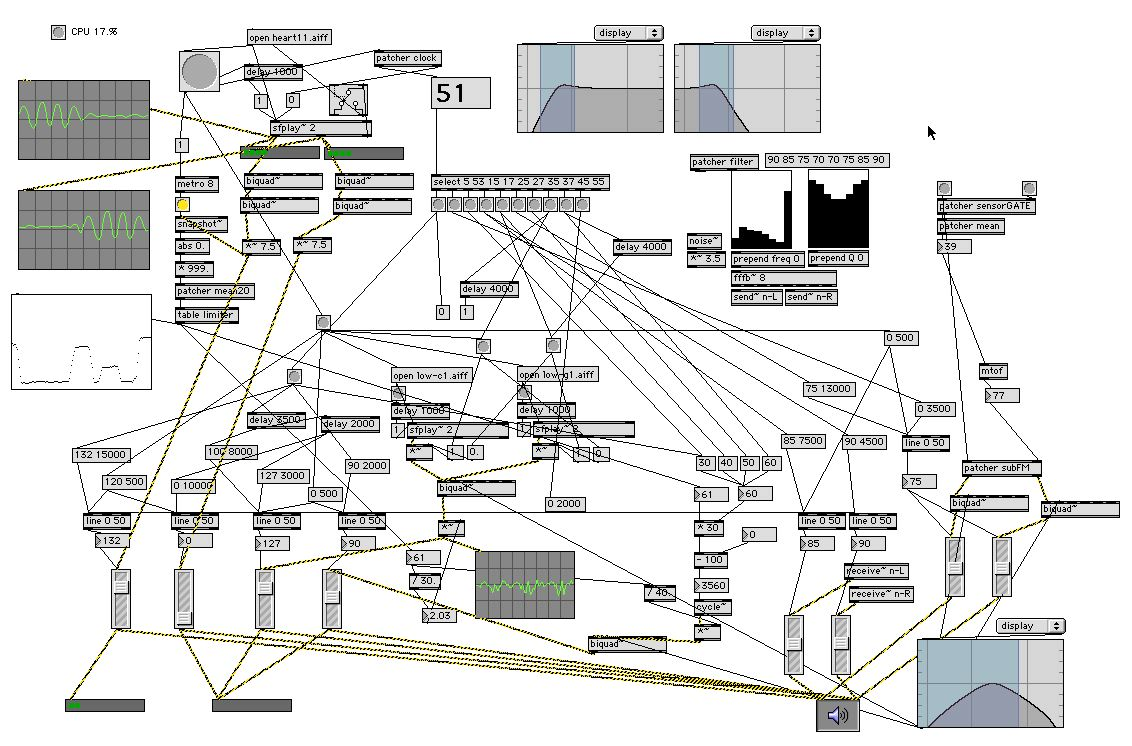
\includegraphics[height=2.25in]{assets/include-max.jpg}
    \caption{Max/MSP: spaghetti code as cautionary tale or design goal?}
    \end{centering}
    \end{figure}
\end{frame}